\normaltrue \difficilefalse \tdifficilefalse
\correctionfalse

%\UPSTIidClasse{11} % 11 sup, 12 spé
%\newcommand{\UPSTIidClasse}{12}

\exer{Banc Balafre $\star$ \label{C2:08:50}}
\setcounter{question}{0}\UPSTIcompetence[2]{C2-08}
\index{Compétence C2-08}
\index{Torseur dynamique}
\index{Banc Balafre}
\ifcorrection
\else
\marginnote{\textbf{Pas de corrigé pour cet exercice.}}
\fi




\ifprof
\else
La figure suivante représente le paramétrage permettant de modéliser les actions mécaniques
s’exerçant sur l’ensemble $S=\{JR+CB\}$. On nommera $G$ le centre d’inertie de l’ensemble
$S$.


\begin{figure}[H]
\centering
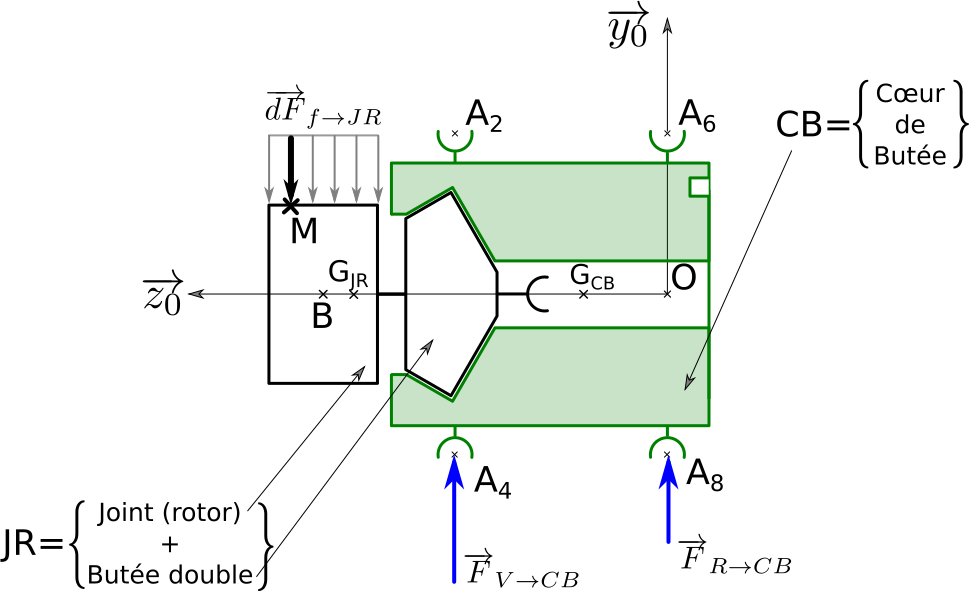
\includegraphics[width=\linewidth]{50_01}
\end{figure}

\textbf{Données et hypohèses}

\begin{itemize}
\item On note $\vect{BM}=z\vect{z_0}+R_J\vect{u}\left(\theta\right)$ où $R_J$ est le rayon du joint avec $R_J = \SI{175}{mm}$;
\item la longueur du joint est $L_J = \SI{150}{mm}$. La position du point $B$, centre du joint est $\vect{OB}=z_B\vect{z_0}$ avec $z_B = \SI{425}{mm}$;
\item Le coeur de butée a une masse $M_{CB} = \SI{40}{kg}$ et la position de son centre d’inertie $G_{CB}$ est paramétrée par $\vect{OG_{CB}}= L_{CB}\vect{z_0}$ avec $L_{CB} = \SI{193}{mm}$;
\item L’ensemble $JR=\{\text{Joint(rotor)+ Butée double}\}$ a une masse $M_{JR} = \SI{100}{kg}$ et la
position de son centre d’inertie $G_{JR}$ est paramétrée par $\vect{OG_{JR}}=L_{JR}\vect{z_0}$ avec $L_{JR}=
\SI{390}{mm}$. On notera $\inertie{G_{JR}}{JR} = \matinertie{A_{JR}}{B_{JR}}{C_{JR}}{-D_{JR}}{-E_{JR}}{-F_{JR}}{\mathcal{B}_{JR}}$ la matrice d’inertie de l’ensemble $JR$ au point $G_{JR}$ exprimée dans une base $\mathcal{B}_{JR} = \left(\vect{x_{JR}},\vect{y_{JR}},\vect{z_{0}}\right)$ liée à $JR$ ;
\item Les positions des points $A_4$ et $A_8$ sont paramétrées par $\vect{OA_4} = z_4\vect{z_0}-R_{CB}\vect{y_0}$ et
$\vect{OA_8}=-R_{CB}\vect{y_0}$ avec $z_4 = \SI{280}{mm}$ et $R_{CB}=\SI{150}{mm}$.
\end{itemize}



Pour simplifier l’étude, on s’intéresse au mouvement généré uniquement dans le plan 
$\axe{y_0}{z_0}$, lorsque les actionneurs 4 et 8 sont commandés en phase, et en opposition de
phase avec les actionneurs 2 et 6. Pendant ce mouvement, les actionneurs 1, 3, 5 et 7 sont
laissés libres. On considérera donc qu’ils n’ont aucune action sur le coeur de butée.

\fi


\question{Décrire la nature du mouvement obtenu pour le coeur de butée CB
par rapport au bâti 0 dans ces conditions.}
\ifprof
\else
\fi

\ifprof
\else

Les actionneurs sont utilisés uniquement pendant les phases de mesure. L’ensemble JR a
donc un mouvement de rotation uniforme par rapport au coeur de butée. On donne les
torseurs cinématiques (exprimés dans le repère lié au bâti $\repere{O}{x_0}{y_0}{z_0}$) : 
$\torseurcin{V}{JR}{CB} =\torseurl{\vecto{JR}{CB}=\Omega\vect{z_0}}{\vect{0}}{G_{JR}}$ avec $\Omega$ constante.
$\torseurcin{V}{CB}{0} =\torseurl{\vect{0}}{v(t)\vect{y_0}}{G_{CB}}$.

La fonction $v(t)$ représente la vitesse de translation du coeur de butée par rapport au bâti.
On peut donc relier $v(t)$ aux déplacements $y(t) = y_4(t) = y_8(t)$ provoqués en $A_4$ et $A_8$
par les actionneurs 4 et 8.
On isole l’ensemble S= \{ JR + CB\} afin de quantifier les efforts dans les actionneurs.
\fi

\question{Exprimer $v(t)$ en fonction de $y(t)$.}
\ifprof
\else
\fi

\question{Déterminer l’expression en $G_{CB}$ du torseur dynamique de CB par
rapport au bâti 0 (fixé au sol et donc considéré comme un référentiel galiléen).}
\ifprof
\else
\fi

\question{Déterminer l’expression en $G_{JR}$ du torseur dynamique de JR par
rapport au bâti 0 (fixé au sol et donc considéré comme un référentiel galiléen).}
\ifprof
\else
\fi

\question{Exprimer alors en $G$ le torseur dynamique de l’ensemble $S$ par rapport
à 0 en fonction de $\dot{v}(t)$, $M_{CB}$ et $M_{JR}$.}
\ifprof
\else
\fi



\ifprof
\else
\begin{flushright}
\footnotesize{Corrigé voir \ref{C2:08:50}.}
\end{flushright}%
\fi